\documentclass{report}
\usepackage{graphicx}
\usepackage{xepersian}
\usepackage{geometry}
\settextfont[Scale=1.2]{XB Zar}
\renewcommand{\baselinestretch}{1.8}

% absolute position title
\usepackage{textpos}

% section numbering
\renewcommand{\thesection}{\arabic{section}}
\renewcommand{\thesubsection}{\thesection.\arabic{subsection}}
\renewcommand{\thesubsubsection}{\thesection.\arabic{subsection}.\arabic{subsubsection}}

\title{
\begin{normalsize}
به نام خدا
\end{normalsize}
\\[2cm]
بررسی مقاله
\\[1cm]
واسنجی مقاوم دوربین برای ویدئوهای ورزشی با استفاده از مدل زمین ورزشی
}
\author{یاسر سوری
\\
\\ \small دانشگاه صنعتی شریف
\\ \small souri@ce.sharif.edu
}
\begin{document}
\maketitle
%\begin{textblock*}{15cm}(0cm,-8cm)\centering به نام خدا \end{textblock*}

\begin{abstract}
در این مقاله روشی برای بدست آوردن ماتریس هوموگرافی بین صفحات زمین و تصویر دوربین، برای تصاویر ورزشی که مدل زمین آن‌ها را می‌دانیم بیان شده است. مانند بسیاری از مقالات دیگر، این مقاله یک مرحله مقدار دهی اولیه برای پارامترهای دوربین دارد و بعد از آن برای هر فریم جدید، دوربین را دنبال  می‌کند\LTRfootnote{tracking}. همچنین فرض شده است که مدل زمین شامل حداقل دو خط افقی موازی و دو خط عمودی موازی است. برای همین الگوریتم برای تصاویر مرکز زمین فوتبال پاسخ‌گو نیست. از دیگر فرضیات مهم این مقاله ثابت بودن مکان و \lr{lens distortion} دوربین در طول زمان است.
\\
لازم به ذکر است که نویسنده این مقاله، در سال بعد ورژن بعدی راه حلش را در مقاله‌ای دیگری چاپ کرده است\cite{new_paper}. مقاله‌ی جدیدتر از لحاظ الگوریتم کلی، فرق زیادی با این مقاله فعلی ندارد. ولی هر کدام از اجزای الگوریتم مقاله‌ی کنونی را به نحوی جایگزین کرده است که الگوریتم برای پردازش برخط به سرعت کافی برسد.

\end{abstract}

\section{فرض‌های مسئله}
در این بخش بعضی از فرضیات مسئله‌ای که قرار است در این مقاله حل شود مورد بررسی قرار می‌گیرد.
\begin{itemize}
\item
فرض شده است که، پارامتر‌های هشتگانه ماتریس هوموگرافی بین زمین و تصویر دوربین را بدست می‌آوریم، و پارامترهای \lr{pan}، \lr{tilt} و \lr{zoom} به صورت مجزا محاسبه نمی‌شوند.
\item
همچنین، پارامترهای مکان دوربین، \lr{roll} و \lr{lens distortion} در طول زمان تغییر نمی‌کنند.
\item
مدل زمین ورزشی (شامل خط‌های زمین، طول و فاصله‌ی آن‌ها از هم) را می‌دانیم.
\item

\end{itemize}
\subsection{نکات}
\begin{itemize}
\item
در این مقاله و مقاله‌های مشابه آن (آن‌هایی که ماتریس هوموگرافی را بدست می‌آورند مثل \cite{new_paper} و \cite{tunesiha}) فرض شده است که مکان دوربین ثابت است، ولی مکان آن را نمی‌دانیم. در حالی که در مقاله \cite{thomas.2007}و دسته‌ مقالات مشابه آن، فرض شده است که مکان دوربین ثابت است، ولی یا مکان آن را می‌دانیم یا روشی برای پیدا کردن مکان آن باید ارائه شود، که معمولا کار سختی است و گاها مراحل غیر خودکار دارد.
\end{itemize}
\section{کلیت روش}
این مقاله دارای دو الگوریتم متفاوت است:
\begin{itemize}
\item
\textbf{مقداردهی اولیه‌ی پارامترهای دوربین}: خروجی این قسمت ماتریس هوموگرافی است. در مقاله بیان شده است که حدود ۱ ثانیه هم به زمان نیاز دارد.
\item
\textbf{دنبال کردن}: در این قسمت، مارتیس هوموگرافی کنونی و لحظه‌ی قبل را استفاده می‌کند و حدسی در مورد ماتریس هوموگرافی لحظه‌ی بعد می‌زند. سپس با استفاده از یک مرحله سریع بهینه‌سازی این حدس را بهبود می‌بخشد. در مقاله بیان شده است که این الگوریتم سریع است و به صورت بلادرنگ می‌تواند اجرا شود.
\end{itemize}
همچنین این مقاله دارای چهار قسمت اصلی است:
\begin{itemize}
\item
پیدا کردن پیکسل‌های سفید که احتمالا بر روی خطوط مدل زمین قرار دارند.
\item
استخراج‌های خطوط مستقیم کاندید برای خطوط مدل زمین.
\item
پیدا کردن سازگاری مناسب بین خطوط کاندید و خطوط مدل. این مرحله بیش‌ترین زمان را می‌برد.
\item
بهبود پارامترهای دوربین.
\end{itemize}
\begin{figure}
\centering
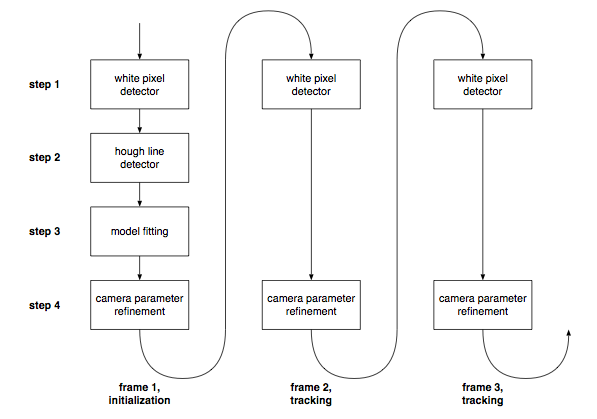
\includegraphics[scale=0.5]{steps.png}
\caption{الگوریتم کلی}
\label{overview}
\end{figure}
برای هر دنباله‌ای از تصاویر مانند شکل \ref{overview} ابتدا در فریم اول، مقداردهی اولیه پارامترهای دوربین (الگوریتم اول) انجام می‌شود که شامل هر چهار قسمت نام برده شده در بالاست. سپس در فریم‌های بعدی الگوریتم دنبال کردن استفاده می‌شود که شامل مرحله‌ی پیدا کردن پیکسل‌های سفید روی خط و بهبود پارامترهای دوربین است.

\subsection{مدل زمین}
فرض شده است که زمین‌های ورزشی، به صورت صفحه هستند. به همین خاطر نگاشت بین مختصات دنیای واقعی و مختصات تصویر یک نگاشت هوموگرافی\LTRfootnote{Homography} است. برای پیدا کردن پارامترهای این ماتریس نیاز به حداقل ۴ نقطه‌ی متناظر داریم. در این مقاله از نقاط تلاقی خطوط زمین به عنوان این نقاط متناظر استفاده شده است.
\subsection{جستجو}
در الگوریتم جستجو ما فرض می‌کنیم که ما پارامترهای ثابت دوربین‌ها را داریم. سپس برای یک تصویر پارامترهایی که تغییر می‌کنند را (ماتریس دوران و فاصله‌ی کانونی) محاسبه می‌کنیم. این محاسبه می‌تواند به خودی خود برای دوربین‌های ثابت مورد استفاده قرار بگیرد یا برای مقدار دهی اولیه در عملیات دنبال‌کردن دوربین‌های مورد استفاده قرار گیرد. از این به بعد فرض می‌کنیم که فاز جستجو برای مقدار دهی اولیه مورد استفاده قرار می‌گیرد.

برای مقدار دهی اولیه زاویه‌های \lr{pan} و \lr{tilt} و مقدار فاصله‌ی کانونی برای یک تصویر خاص، ابتدا فرض می‌کنیم که از تصویر ورودی را تبدیل به تصویر باینری کرده‌ایم که در آن نقاطی که ممکن است روی خطوط قرار داشته باشند در آن مشخص شده است. مرحله‌ی تشخیص خطوط از تبدیل هاف\LTRfootnote{Hough transform} استفاده می‌کند با این تفاوت که تصویر را به ۱۰ قسمت مساوی (عمودی یا افقی، بسته به نزدیک به عمودی یا نزدیک به افقی بودن خطوط زمین) تقسیم می‌کند و برای هر کدام از آن قسمت‌ها یک تبدیل هاف جدا را محاسبه می‌کند. لازم است که توجه کنید برای هر بار مقدار دهی اولیه، یک بار تبدیل هاف تصویر حساب می‌شود.

سپس برای مقادیر مختلف ممکن از پارامترهای \lr{pan}، \lr{tilt} و فاصله‌ی کانونی با اندازه‌ی گام مشخصی، مدل زمین را بر روی تصویر می‌اندازیم. حال برای هر خط از خطوط مدل زمین که در تصویر قابل رؤیت است، بسته به اینکه در کدام نواحی ۱۰ گانه در تقسیم بندی قرار دارد، نقطه‌ی معادل را در فضاهای هاف ده‌گانه پیدا می‌کنیم و مقدار آن نقطات را در فضای هاف برای تمام خطوط زمین با یکدیگر جمع می‌کنیم. حاصل این جمع به ما ارزش این پارامترهای دوربین را می‌دهد.

در انتهای جستجو از بین تمام پارامترهای مختلف دوربین، آن ۱۰ تایی را انتخاب می‌کنیم که دارای ارزش بیش‌تری هستند. در مراحل دنبال کردن دوربین در حقیقت ۱۰ دنبال کردن همزمان را انجام می‌دهیم. ولی پس از چند مرحله از دنبال کردن مشخص می‌شود که فقط یکی از این مقادیر خوب دنبال می‌شود و آن را انتخاب می‌کنیم. همچنین باید توجه کنیم که در انتخاب ۱۰ تا از سه‌تایی پارامترهای \lr{pan}، \lr{tilt} و فاصله‌ی کانونی که دارای بیش‌ترین ارزش هستند، از انتخاب مقادیر نزدیک به هم که عملا ماکزیمم‌های محلی هستند اجتناب می‌کنیم و آن‌هایی را انتخاب می‌کنیم که دارای تفاوت حداقلی در زوایا باشند.
\subsection{دنبال کردن}
در مرحله‌ی دنبال کردن، ما یک حدس اولیه از پارامترهایی دوربین که همان مقادیر زمان (فریم) قبل هستند را داریم و حال می‌خواهیم برای فریم جدیدی که دوربین تصویر آن را ضبط کرده است، پارامترهای جدید را بدست آوریم. این مرحله در حقیقت یک روش بهینه‌سازی گام به گام \LTRfootnote{iterative} است که می‌توان آن را برای پارامترهای ثابت، متحرک یا هر دو دسته پارامترهای دوربین حل کرد. برای اطلاع از جزئیات بیش‌تر این قسمت به خود مقاله مراجعه کنید.
\section{موارد مبهم}
این مقاله دو قسمت مبهم برای من دارد:
\begin{itemize}
\item
اول در مرحله‌ی تعیین شیب زمین و موقعیت دوربین، چگونه مسئله‌ی بهینه سازی را حل می‌کند؟
\item
دوم اینکه در مرحله‌ی جستجو، گام را به چه طریقی تعیین کرده است؟
\end{itemize}
\section{پیاده‌سازی}
به نظر می‌رسد که این مقاله و راه حلی که ارائه داده است، قابلیت حل کردن مسئله‌ی ما را داشته باشد. از آنجایی که در صورت مسئله‌ی ما، موقعیت دوربین‌ها تعیین شده است، در فازهای اول پیاده‌سازی این مقاله نیازی به انجام دادن این کار نیست.

ضمنا اکثر دوربین‌های ما ثابت هستند. این مسئله هم یک حسن است و هم یک عیب. حسن از این نظر که برای واسنجی این دوربین‌ها نیازی به پیاده‌سازی مرحله‌ی دنبال کردن نداریم. و عیب از این نظر که در روش این مقاله خروجی مرحله‌ی جستجو ۱۰ سری پارامتر برای دوربین است که در مرحله‌ی دنبال کردن بهترین آن‌ها تعیین می‌شود که از آنجایی که دوربین ما تکان نمی‌خورد، ما نمی‌توانیم بهترین سری پارامترها را با روش این مقاله انتخاب کنیم. پس باید فکری به حال انتخاب بهترین سری پارامترها بکنیم.

\renewcommand{\baselinestretch}{1}
\renewcommand*{\refname}{\section{منابع}}

\begin{latin}
\bibliography{court_model_bib}{}
\bibliographystyle{plain}

\end{latin}

\end{document}